\section{Casos de Estudio}
\label{sec:casos_de_estudio}
 
 El desarrollo iterativo del framework implicó la ejecución de pruebas con cada versión del framework obtenida. El mismo ha sido probado y validado empleando dos aplicaciones de escritorio JMoney (http://jmoney.sourceforge.net/) y Freemind (http://freemind.sourceforge.net/). 
 
%\begin{description}
%
%\item[JMoney]
%
%%Es un gestor de finanzas de uso personal. Tiene ??? paquetes, 83 clases, 594 métodos y 436 atributos. Se compone de 5780 líneas de código. 
%
%\item[Freemind]
%
%%Es una herramienta para la creación de mapas mentales. Tiene 50 paquetes, 820 clases, 6974 métodos, 2816 atributos. Se compone de 108.378 líneas de código. 
%\end{description}

Para cada una se crearon diversas tareas y en cada iteración se configuró el framework. Los principales objetivos de las pruebas fueron constatar que el registro de los datos y cálculo de las métricas funcionaba correctamente; y comprobar el nivel de reúso, configuración y especialización. A continuación se presenta una tarea para cada caso de estudio, el aspecto que fue adaptado  y el resultado de las pruebas.


\begin{description}

\item[Freemind]
Tarea: Crear Mapa Mental Básico.

	\begin{enumerate}
		\item Crear un nuevo mapa, haciendo clic en el botón "Nuevo" desde la barra de herramientas, o desde el menú Archivo. 
		\item Completar el texto del nodo raíz del mapa creado.
		\item Construir una jerarquía de tres niveles con nodos hijos y hermanos (al menos 11).Para ello se deberá posicionar en el nodo sobre el cual quiere crear un nodo hijo o hermano y luego insertar el nodo desde las opciones del menú contextual, o desde el menú Insertar.
		\item Ir al menú herramientas y ordenar los nodos por nombre.
		\item Guardar el mapa mental en el escritorio con un nombre significativo.
	\end{enumerate}
	
%	\begin{itemize}
%		\item Inicio de la tarea: La tarea se considerará iniciada luego que el usuario haya seleccionado la opción "Nuevo Mapa" del menú principal o desde la barra de herramientas.
%		\item Fin de la tarea: La tarea se considerará finalizada luego que el usuario guarda, por primera vez, el mapa en un archivo con el nombre solicitado. 
%	\end{itemize}
	
	\begin{verbatim}
	public aspect FreemindTask1extends TaskConnect{
	 private String idTask="Crear Mapa Conceptual Básico”;
	 pointcut startTask():execution(void  
	 freemind.modes.common.actions.NewMapAction.	\\
	 actionPerformed(ActionEvent));
	 pointcut endTask():execution( 	 
	  *freemind.modes.ControllerAdapter.SaveAsAction.*(..)) ||
	    execution(* freemind.modes.ControllerAdapter.\\
	    SaveAction.*(..));
	}
	\end{verbatim}

	%insertar fig4.png
	\begin{figure*}[ht!]
		\centering
		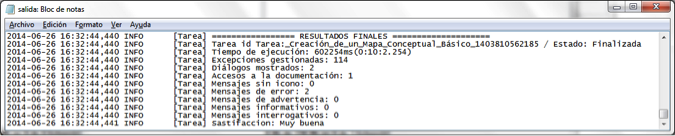
\includegraphics[scale=1]{figs/fig4.png}
		\caption{\label{fig:fig4} Log de Tarea: Crear Mapa Conceptual Básico.}
	\end{figure*}

\item[JMoney]
Tarea: Crear una nueva cuenta

	\begin{enumerate}
		\item Hacer click en el botón derecho del panel lateral y seleccionar la opción "new account".
		\item Ingresar las propiedades de la cuenta desde el panel properties de la cuenta
		\item Ingresar entradas en la cuenta desde el panel entries  
		\item Salvar desde el botón "save" en la barra de herramientas o desde menú "file/save", usando combinación de teclas "ctrl+s" o respondiendo afirmativamente al mensaje de grabar los cambios antes de cerrar la aplicación.
	\end{enumerate}

	\begin{verbatim}
		public aspect Tarea1JMoneyConnect extends TareaConnect{		
		     private String idTask=”Crear Nueva Nuenta”;
		     pointcut starTask():execution(void   
		                  net.sf.jmoney.gui.MainFrame.newAccount());
		     pointcut endTask():execution(void                  
		               net.sf.jmoney.gui.MainFrame.saveSession()) || 
		       execution(void net.sf.jmoney.gui.MainFrame.saveSessionAs());
	}
	\end{verbatim}

	%insertar fig5.png
	\begin{figure*}[ht!]
		\centering
		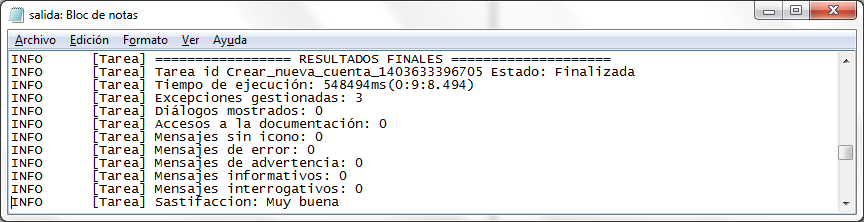
\includegraphics[scale=1]{figs/fig5.png}
		\caption{\label{fig:fig5} Log de Tarea: Crear Nueva Cuenta.}
	\end{figure*}
	
\end{description}